%!TEX root = ../username.tex
\chapter{The Software} \label{software}

This chapter discusses the various components of the software used in this project.
All components use \texttt{music21}, a Python library for music developed by MIT, to handle input and output of music notation to and from a Python-native format.
Input files are in MIDI format.

\section{Overview} \label{software:overview}

The data flow for the set of programs used in this project are as follows:
Optionally, the Markov chain program reads a corpus of music to create its transition matrices.
Because good music exists in many keys, when reading the corpus of music, we normalize all the music to the key of C Major or A Minor.
These keys are chosen because their key signature contains no sharps and no flats.
We also cache the normalized corpus, so we do not need to go through the process of determining the key of a piece and transposing it every time we run the program.
These Markov chains are then used to produce the initial population for the genetic algorithm.
If we choose not to use the Markov chain program to generate the initial population, we use a randomly generated initial population instead.
The genetic algorithm uses an LSTM neural network (see Section \ref{ga:fitness}) as a surrogate fitness function, which was trained with its own music corpus.
See Figure \ref{fig:softwareoverview} for a visual representation of the broad flow of data.

\begin{figure}[h]
	\centering
	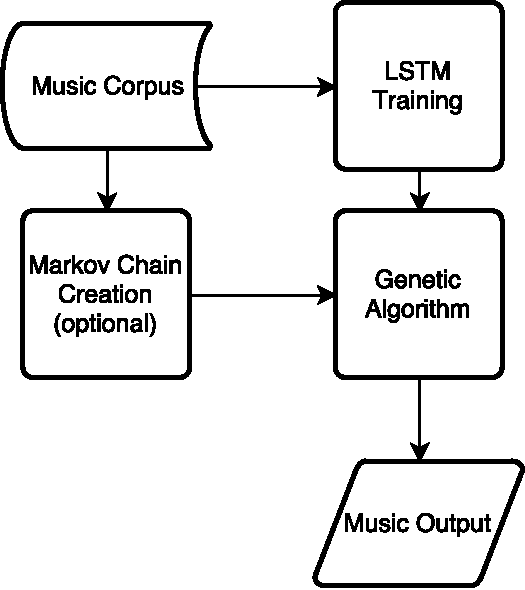
\includegraphics{figures/overview_flowchart.pdf}
	\caption{The flow of data through the software.}
	\label{fig:softwareoverview}
\end{figure}

\section{Markov Melody Generator} \label{software:markov}

In the code repository for this project, the directory \texttt{intervalMarkovChain} contains Python code to generate melodies using Markov chains of arbitrary order.
The theory behind this software component is discussed in Section \ref{bg:markov} and Chapter \ref{markov}.
The software uses two Markov chains to generate a melody: one for the intervals between notes and the other for rhythms of notes.
See Figure \ref{fig:markovflowchart} for a visual representation of the flow of data through the Markov melody generation.

\begin{figure}[h!]
	\centering
	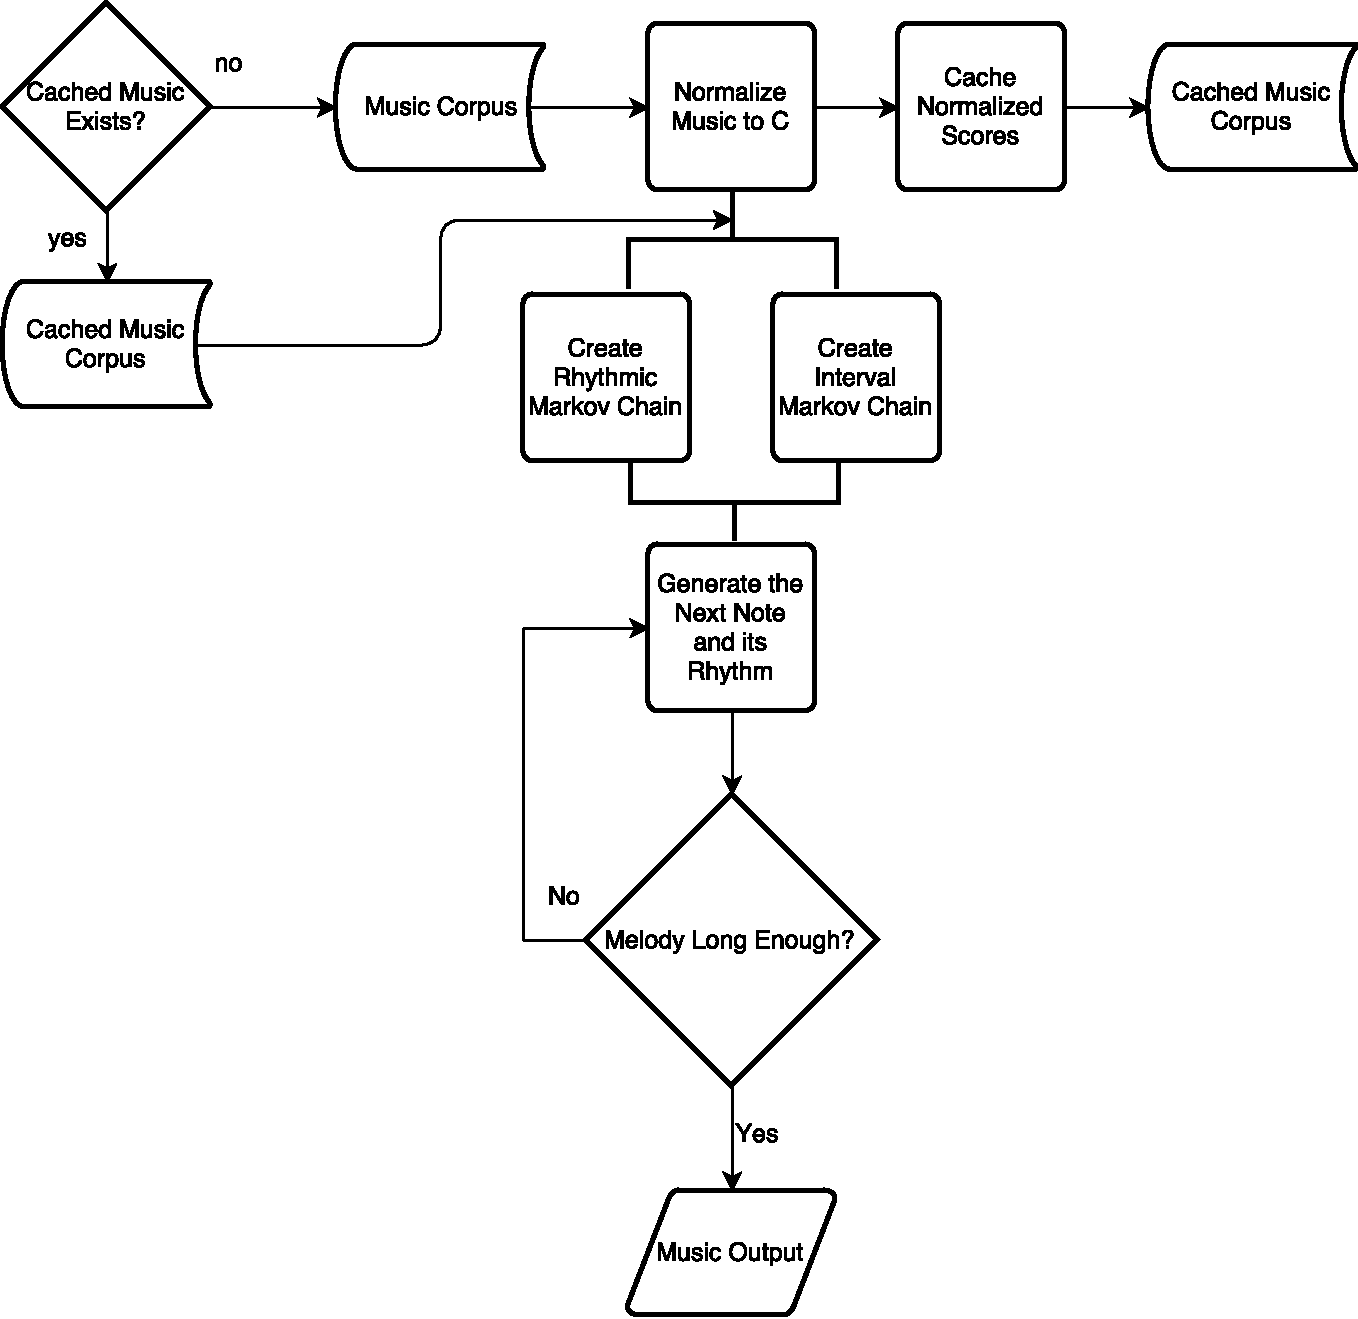
\includegraphics[width=\linewidth]{figures/markov_flowchart.pdf}
	\caption{The flow of data through the creation of a Markov melody.}
	\label{fig:markovflowchart}
\end{figure}

In order to facilitate the creation of Markov chains in a more general way, we create a \texttt{MarkovChain} object, which provides methods to create and use the Markov chain.
When a \texttt{MarkovChain} object is created, it requires an order to use.
By default, the order is $1$.
To create the transition matrix, the function \texttt{create\_transition\_matrix(streams, chainType)} accepts a list of the \texttt{music21} \texttt{Streams} to use as the training source, as well as what type of Markov chain it should be -- should it calculate transition probabilities for rhythms or for the intervals between notes?

An $n$th order Markov chain is represented using \texttt{defaultdict}s nested $n + 1$ deep.
Two interesting functions in this class are \texttt{arbitrary\_depth\_dict\_get} and \texttt{arbitrary\_depth\_dict\_set}.
These functions allow one to read from and write to \texttt{dict}s of arbitrary depth.
These are necessary to be able to create and use the transition matrices because the order of the Markov chain may not always be the same, so the number of index operators desired cannot be hard-coded.

The function \texttt{arbitrary\_depth\_dict\_get(subscripts, default, nested\_dict)} works by recursively accessing \texttt{nested\_dict} with the first element of \texttt{subscripts} until either \texttt{subscripts} is empty or a key from \texttt{subscripts} does not exist.
In the former case, the function returns the value of \texttt{nested\_dict} specified by \texttt{subscripts}.
In the latter case, the function returns the specified default value.

The function \texttt{arbitrary\_depth\_dict\_set(subscripts, \_dict, val)} works by iterating through the \texttt{subscripts} of \texttt{\_dict}, going a level deeper at each step.
At each level, an empty dictionary is created if one did not already exist at that index.
This function makes use of the fact that the \texttt{dict} data structure in Python can be assigned to a new variable by reference in order to go into the next index.
On the final index, the dictionary is assigned the value at the (possibly nested) index as specified by \texttt{subscripts}.

The \texttt{MarkovChain} class is implemented in \texttt{intervalMarkovChain/markovChain.py}.

In order to create a Markov chain, we need a corpus with which to build it.
Conveniently, \texttt{music21} provides the ability to read and write a variety of file formats.
In this project, we use MIDI files to store the music we use as a corpus and that we generate.

Because a Markov chain requires some predetermined seed notes to refer to, the first four notes of each generated melody are C, D, E, and D.
These pitches were chosen because the intervals between them (Major seconds up and down) will appear in almost any corpus of music at least once.
To keep some rhythmic diversity, the duration for each of these four notes is randomly chosen to be a sixteenth note, eighth note, or quarter note.
The decision to include four seed notes was subjectively made by the author's thoughts that melodies produced using a fourth order interval Markov chain were not sufficiently better than melodies produced using a third order chain to warrant the extra computational cost.
In order to use a Markov chain with an order higher than four, more seed notes must be provided.

Once the interval and rhythm Markov chains are generated and we have our seed notes, we can generate a melody.

The process of reading reading a corpus of music, creating the Markov chains, and generating a melody is implemented in \texttt{intervalMarkovChain/intervalMarkovChain.py}.

\section{Genetic Algorithms} \label{software:ga}

The directory \texttt{geneticAlgorithms} contains Python code to manipulate existing melodies with genetic algorithms to produce better output.
The theory behind this software component is discussed in Section \ref{bg:ga} and Chapter \ref{ga}.

\subsection{Fitness Function} \label{software:ga:fitness}

This program uses an LSTM neural network created using \texttt{TensorFlow} as a surrogate fitness function.
\texttt{TensorFlow} is a machine learning library for Python developed by the Google Brain team.
The file \texttt{geneticAlgorithms/lstm.py} contains code to convert music data to a form usable by the artificial neural network, train the LSTM neural network on that modified music data, and save the generated model for later use.
See Figure \ref{fig:lstmflowchart} for the flow of data through the creation of the fitness function.

\begin{figure}[h!]
	\centering
	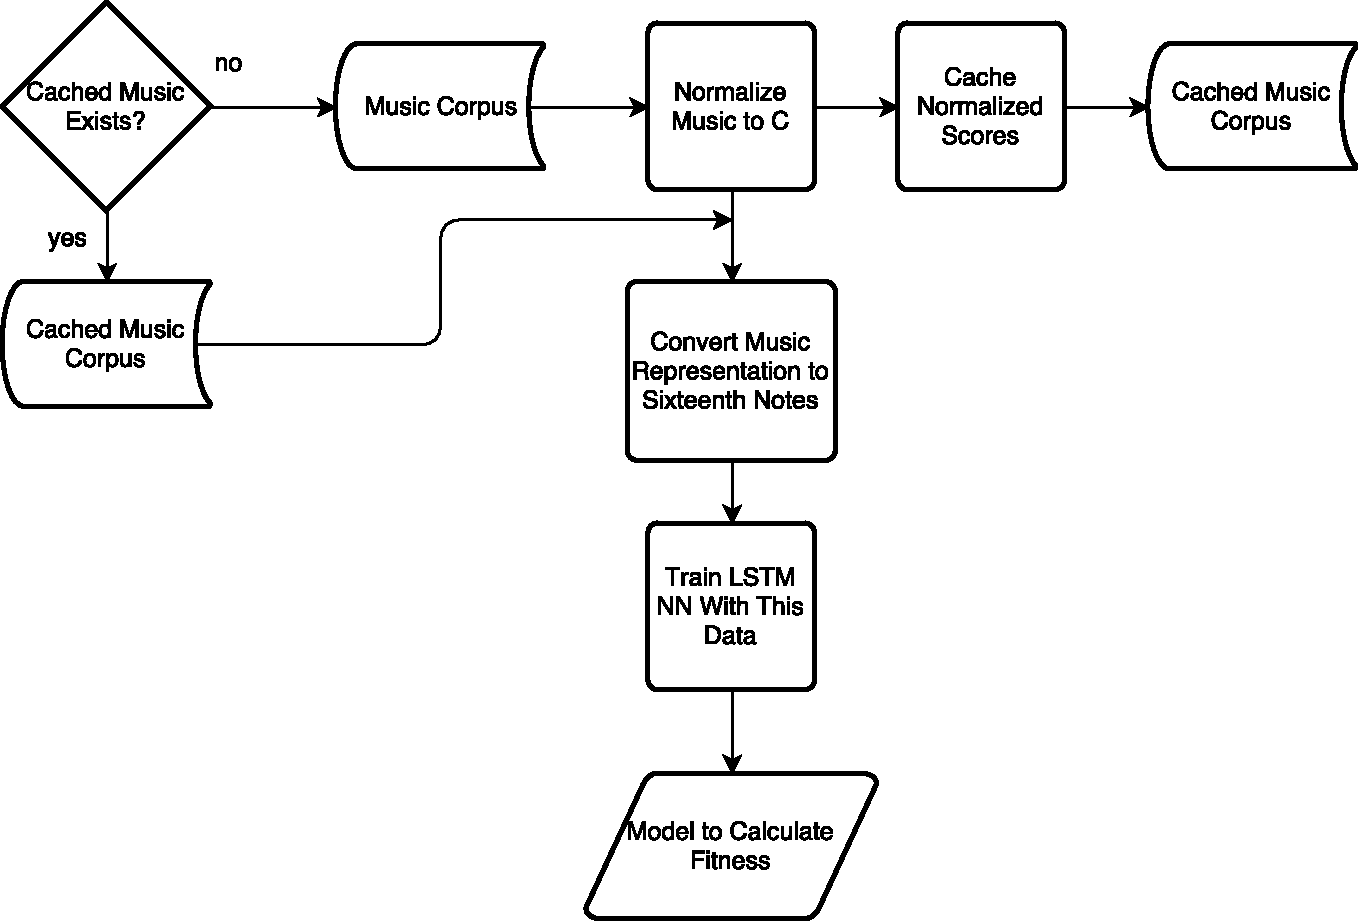
\includegraphics[width=\linewidth]{figures/lstm_flowchart.pdf}
	\caption{The flow of data through the creation of the LSTM neural network to use as the surrogate fitness function.}
	\label{fig:lstmflowchart}
\end{figure}

The first step is to read a corpus of music to train the function on.
If no music corpus is provided, the program uses the collection of Bach chorales that come with \texttt{music21}.
As with the Markov chain module, this module normalizes the melodies to the key of C before training, using cached copies of the normalized scores if they are available.
This removes the need to take the key a piece is into account.

After the training input is normalized it is converted to a form the artificial neural network will be able to recognize.
We perform some preprocessing by one-hot encoding the pitch of each note.
To limit the range of octaves that can appear in our music, we use the MIDI values for each pitch.
Because the MIDI standard defines values from $0$ to $127$, we can \textit{one-hot encode} the pitch as an array of zeros with a $1$ at the index of the MIDI number we want to represent.
One-hot encoding is a method used in data science to represent categorical data in a numeric format.
Even though the MIDI values are already numeric, we one-hot encode them because the difference of a half step (one MIDI value) can be the distinction between a good melody and a better melody.
Additionally, MIDI values are only ever integer values, so we do not need to represent them as floats.
Importantly, one-hot encoding the MIDI values improves the accuracy of the network.
Now that the good music data is in a form the neural network can recognize, a number of random sequences of sixteenth notes is generated to act as samples of bad samples.
We want the neural network to train on an evenly distributed sampling of good and bad data, so we shuffle the list.

Now the program is ready to create and train the LSTM network.
Unlike a traditional neural network, an input sample is not entered all at once.
Instead, each note enters the network one at a time.
For this project, we consider four measures of 4/4 music as input to the neural network.
With our rhythmic encoding of sixteenth notes, this means for each music sample we input $16 * 4 = 64$ notes to the network.
In more general terminology, each note is a \textit{chunk}.
Since each note consists of a single one-hot encoded pitch, the \textit{chunk size} is $128$.
Somewhat arbitrarily, we pass each input through $256$ neurons in the network.
The output of the network is an array containing two values, which are the network's certainty that the input is or is not a good melody.

To train the model, we run the training data through a function to reshape it to a $N$ x 64 x 128 list, where $N$ is the number of training samples.
$70\%$ of this reshaped data is then fed through the neural network for five epochs.
That is, the data is fed to the network and weights are adjusted five times.
At this point, the accuracy of the model is found by evaluating the remaining $30\%$ of the training data and comparing the output to the actual labels.
If the accuracy is sufficient, the \texttt{TensorFlow} session and the model are returned to be used on new data later.

Using the \texttt{evaluate\_part()} function, the fitness for a melody is the output of the mathematical squashing function $f(x) = \frac{\arctan(\frac{x}{5}) + \frac{\pi}{2}}{\pi}$, where $x$ is the difference between the outputs of the LSTM neural network.
We use this function to normalize all fitnesses to the range $(0,1)$.
Arctangent naturally has limits of $\frac{-\pi}{2}$ and $\frac{\pi}{2}$, so we add $\frac{\pi}{2}$ to shift the fitness up, then divide by $\pi$ to squash the fitness to less than $1$.
We divide $x$ by $5$ to make the output more uniform across the interval $(0,1)$.
Otherwise, the function approaches $0$ and $1$ too quickly as $x$ moves further from $0$.

\subsection{Mutations} \label{software:ga:mutations}

Section \ref{ga:mutate} contains the theoretical background of these mutations.

Because we are working with music data, there are some specific operations we can perform to act as a type of mutation, as well as crossover.

The six functions we use to operate on \texttt{music21} \texttt{stream} objects are \texttt{transpose()}, \texttt{inverse()}, \texttt{retrograde()}, \texttt{retrograde\_inverse()}, \texttt{inverse\_retrograde()}, and \texttt{crossover()}.

\texttt{transpose(stream, interval)} is simply a wrapper for \texttt{music21}'s \texttt{Stream.transpose()} method.
It accepts a \texttt{Stream} and an amount to transpose by, measured in semitones.

\texttt{inverse(stream)} returns the inverse of \texttt{stream}.
That is, it takes the inverts the intervals between notes.
For example, the sequence CDE becomes CB$\flat$A$\flat$.

\texttt{retrograde(stream, reverse\_notes, reverse\_rhythms)} returns the retrograde version of \texttt{stream}, with the options to reverse the pitches, the rhythms, or both.

\texttt{retrograde\_inverse(stream)} and \texttt{inverse\_retrograde(stream)} are wrapper functions for \texttt{inverse()} and \texttt{retrograde()} together, one for each order.

\texttt{crossover(parent1, parent2, crossover\_points)} provides the ability to perform crossover of two \texttt{Stream}s.
The function returns two new \texttt{Stream}s.
The first \texttt{Stream} we return is obtained by copying notes from \texttt{parent1} until the first index in \texttt{crossover\_points} is reached, then copying notes from \texttt{parent2} until the second index in \texttt{crossover\_points}, and so on, alternating which parent's notes are copied, until there are no more indices in \texttt{crossover\_points}.
The second returned \texttt{Stream} is obtained similarly, but starts by copying notes from \texttt{parent2}.

These functions are implemented in \texttt{geneticAlgorithms/mutations.py}

\subsection{Evolving Melodies} \label{software:ga:evolving}

The file \texttt{geneticAlgorithms/geneticAlgorithms.py} contains code to carry out the genetic algorithm that takes some initial population of melodies, remixes and mutates them, and eventually produces some more fit output as measured by the fitness function.
It uses all of the previously discussed components to achieve this.
See Figure \ref{fig:gaflowchart} for the flow of data through the use of genetic algorithms to generate melodies.

\begin{figure}[h!]
	\centering
	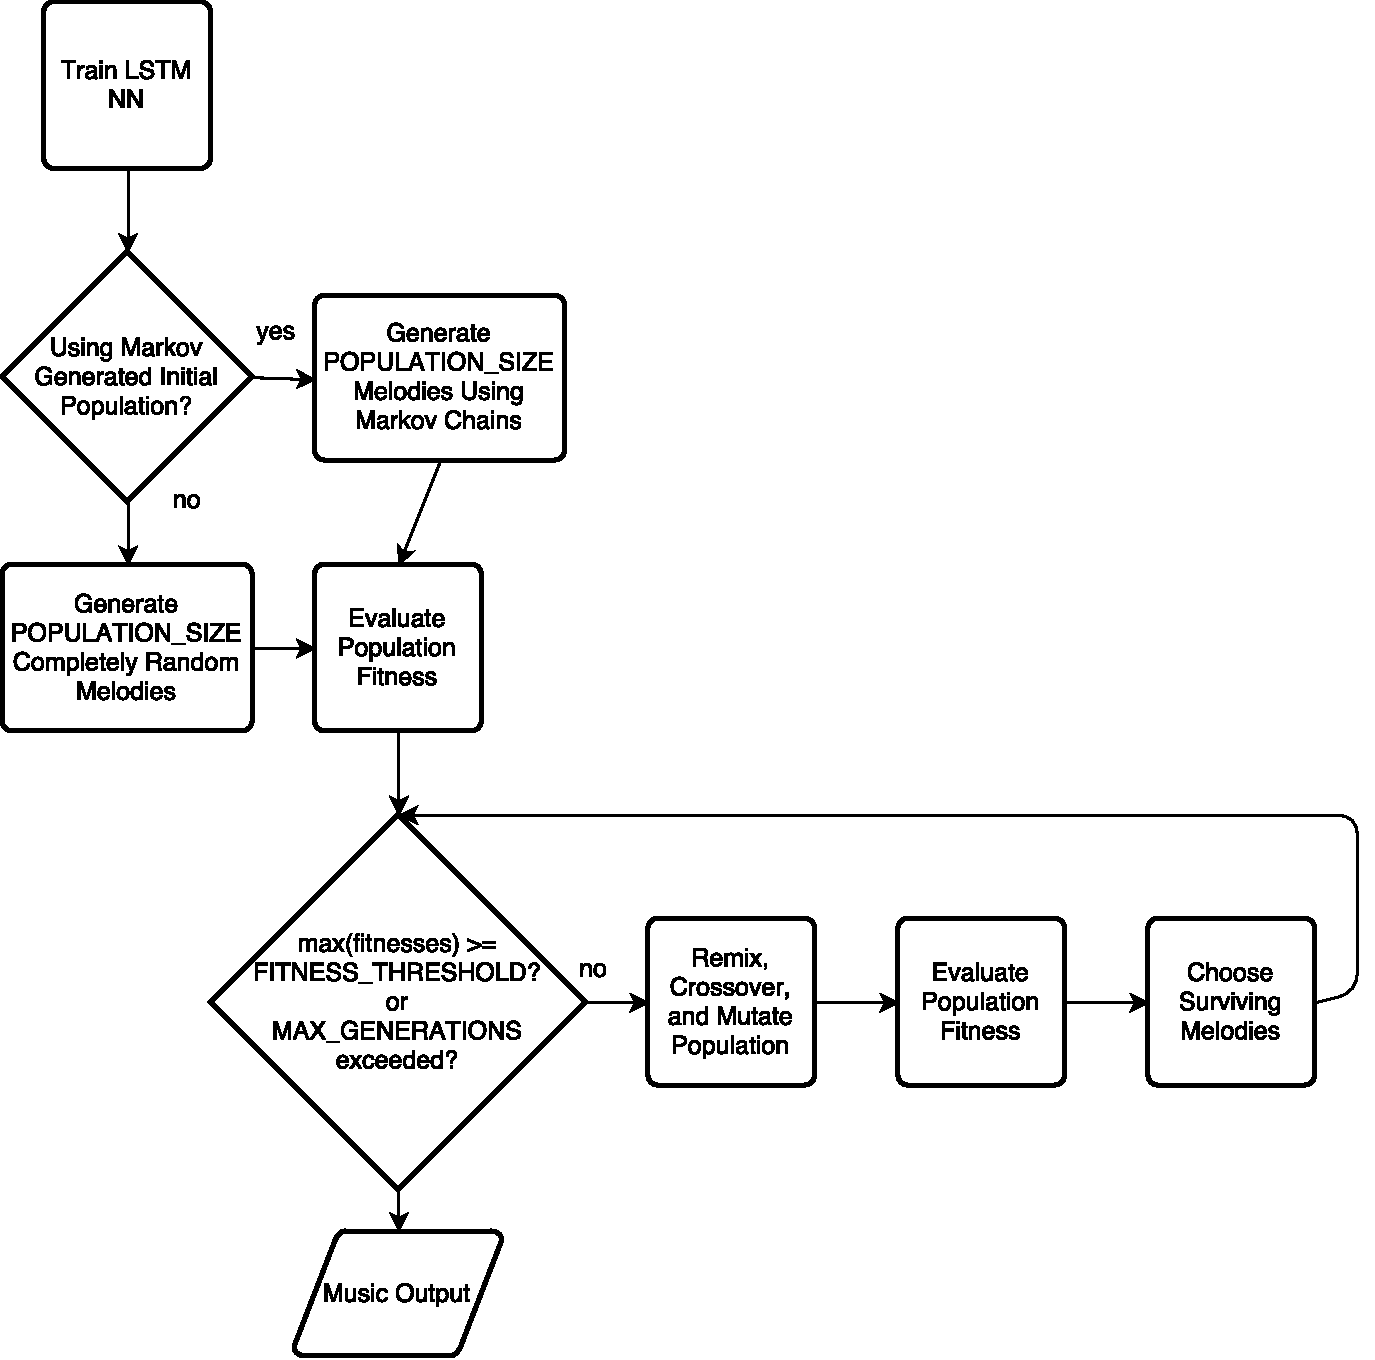
\includegraphics[width=\linewidth]{figures/genetic_algorithm_flowchart.pdf}
	\caption{The flow of data through the use of genetic algorithms to generate melodies.}
	\label{fig:gaflowchart}
\end{figure}

The program starts by creating the fitness function using \texttt{lstm.py}.
Then the initial population is produced.
This can either use \texttt{intervalMarkovChain/intervalMarkovChain.py} to generate the initial population, or it can use completely random music to accomplish this.
Starting with the Markov chain will generally produce an initial population with a higher fitness, but it will take more time to generate the population.
The fitness values of the initial population are calculated while the initial population is being generated.

At this point the program is ready to enter the main loop.
Its stopping conditions are when a melody has a high enough fitness or the maximum number of generations has been reached.
Inside the loop, the program uses a pool of worker processes to remix the population using the functions inside of \texttt{mutations.py}.
% ... uses the \texttt{multiprocess} library from The UQ Foundation \cite{mckerns_better_2018}.
% Rather than the standard \texttt{multiprocessing} library, \texttt{multiprocess} was chosen because \texttt{music21} \texttt{streams} use weak references to relate notes to the streams to which they belong, which Python's \texttt{pickle} library cannot handle.
% \texttt{multiprocess} is a fork of \texttt{multiprocessing} that uses \texttt{dill}, a fork of \texttt{pickle} that allows for weak references.
After this remixing, the loop generates some melodies using crossover, and mutates some of the melodies.
This mutation is to ensure the population does not stagnate.
At this point the loop calculates the fitnesses of the new population, chooses the seed population for the next generation, and goes back to the beginning of the loop.

\section{How to Use the Software} \label{software:howtouse}

\subsection{Markov Melody} \label{software:howtouse:markov}

To produce a melody using the Markov Melody program, call the program \texttt{intervalMarkovChain.py} along with the corpus of music to use, either directly as the MIDI files to use, or as a directory containing MIDI files.
If no corpus is provided, it defaults to any \texttt{.mid} files located in the relative directory \texttt{../corpus}.
From the command line, this might look like

\texttt{python3 intervalMarkovChain.py song1.mid song2.mid}

\noindent when directly specifying the MIDI files to use, or

\texttt{python3 intervalMarkovChain.py}

\noindent to use the default music corpus.
Also, the function \texttt{generate\_melody()}, which handles the creation of melodies inside \texttt{intervalMarkovChain.py}, checks if the parameter \texttt{corpus} is set to \texttt{False}.
In the case that it is \texttt{False}, the function uses the built in \texttt{music21} collection of Bach chorales.
This option is only available when importing the file from another Python script.


\subsection{Genetic Melody} \label{software:howtouse:ga}

Run \texttt{python3 geneticAlgorithm.py} to generate a set of melodies produced by the genetic algorithm.
The program accepts some optional flags:

\noindent -f, -{}-desired-fitness value 

Sets the fitness required to terminate the program to value

\noindent -s, -{}-population-size value

Sets the size of the population of each generation to value

\noindent -g, -{}-max-generations value

Set the maximum number of generation the program will run to value

\noindent -m

Sets the program to use Markov chains to generate the initial population

For example: To use $5000$ generations with a population of $500$ and a desired fitness of $0.9$, with the initial population produced using Markov chains, you could use

\texttt{python3 geneticAlgorithm.py -f 0.9 -g 5000 -s 500 -m}

\noindent or

\texttt{python3 geneticAlgorithm.py -{}-desired-fitness 0.9 -{}-max-generation 5000 -{}-population-size 500 -m}
